
%--------------------------------------------------------------------------
%
%  M.Sc. Thesis
%  [Put Your Thesis Title Here]
%  By: [Put Your Name Here]
%
%--------------------------------------------------------------------------

%--------------------------------------------------------------------------
%
%  LaTeX Thesis Template (v2.2)
%  By: Hamid Zarrabi-Zadeh
%
%  Contributors:
%      Ehsan Emamjomeh-Zadeh
%      Omid Gheibi
%
%--------------------------------------------------------------------------


\documentclass[oneside,a4paper,12pt]{book}
\usepackage{graphics}
\usepackage{booktabs}
\usepackage{makecell}
\usepackage{multirow}
\usepackage{pifont}% http://ctan.org/pkg/pifont
\newcommand{\cmark}{\ding{51}}%
\newcommand{\xmark}{\ding{55}}%

\usepackage{caption} % for modifying the caption format

% Define a command for right-to-left text
\newcommand{\ltr}[1]{\beginL #1\endL}


\newcommand*\rot{\rotatebox{90}}
\newcommand*\OK{\ding{51}}


% -------------------------------------------------------
%  Common Styles and Formattings
% -------------------------------------------------------


\usepackage{amssymb,amsmath}
\usepackage[colorlinks,linkcolor=blue,citecolor=blue]{hyperref}
\usepackage{minitoc} %table of content for each chapter
\usepackage[usenames,dvipsnames]{pstricks}
\usepackage{graphicx,subfigure,wrapfig}
\usepackage{geometry,fancyhdr}
\usepackage[mathscr]{euscript}
\usepackage{multicol}
\usepackage{tabularx}
\usepackage{pdfpages}
\usepackage{algorithmicx,algorithm}

\usepackage[localise=on,extrafootnotefeatures]{xepersian}
\usepackage[noend]{algpseudocode}
\input{styles/alg-fa}



% -------------------- Page Layout --------------------


\newgeometry{top=3.5cm,bottom=3.5cm,left=2.5cm,right=3cm,headheight=25pt}

\renewcommand{\baselinestretch}{1.4}
\linespread{1.6}
\setlength{\parskip}{0.45em}

\fancyhf{}
\rhead{\leftmark}
\lhead{\thepage}


% -------------------- Fonts --------------------

\settextfont[
Scale=1.09,
Extension=.ttf, 
Path=styles/fonts/,
BoldFont=XB NiloofarBd,
ItalicFont=XB NiloofarIt,
BoldItalicFont=XB NiloofarBdIt
]{XB Niloofar}

\setdigitfont[
Scale=1.09,
Extension=.ttf, 
Path=styles/fonts/,
BoldFont=XB NiloofarBd,
ItalicFont=XB NiloofarIt,
BoldItalicFont=XB NiloofarBdIt
]{XB Niloofar}

\defpersianfont\sayeh[
Scale=1,
Path=styles/fonts/
]{XB Kayhan Pook}


% -------------------- Styles --------------------


\SepMark{-}
\renewcommand{\labelitemi}{$\small\bullet$}



% -------------------- Environments --------------------


\newtheorem{قضیه}{قضیه‌ی}[chapter]
\newtheorem{لم}[قضیه]{لم}
\newtheorem{ادعا}[قضیه]{ادعای}
\newtheorem{مشاهده}[قضیه]{مشاهده‌ی}
\newtheorem{نتیجه}[قضیه]{نتیجه‌ی}
\newtheorem{مسئله}{مسئله‌ی}[chapter]
\newtheorem{تعریف}{تعریف}[chapter]
\newtheorem{مثال}{مثال}[chapter]


\newenvironment{اثبات}
	{\begin{trivlist}\item[\hskip\labelsep{\em اثبات.}]}
	{\leavevmode\unskip\nobreak\quad\hspace*{\fill}{\ensuremath{{\square}}}\end{trivlist}}

\newenvironment{alg}[2]
	{\begin{latin}\settextfont[Scale=1.0]{Times New Roman}
	\begin{algorithm}[t]\caption{#1}\label{algo:#2}\vspace{0.2em}\begin{algorithmic}[1]}
	{\end{algorithmic}\vspace{0.2em}\end{algorithm}\end{latin}}


% -------------------- Titles --------------------


\renewcommand{\listfigurename}{فهرست شکل‌ها}
\renewcommand{\listtablename}{فهرست جدول‌ها}
\renewcommand{\bibname}{\rl{{مراجع}\hfill}} 


% -------------------- Commands --------------------


\newcommand{\IN}{\ensuremath{\mathbb{N}}} 
\newcommand{\IZ}{\ensuremath{\mathbb{Z}}} 
\newcommand{\IQ}{\ensuremath{\mathbb{Q}}} 
\newcommand{\IR}{\ensuremath{\mathbb{R}}} 
\newcommand{\IC}{\ensuremath{\mathbb{C}}} 

\newcommand{\set}[1]{\left\{ #1 \right\}}
\newcommand{\seq}[1]{\left< #1 \right>}
\newcommand{\ceil}[1]{\left\lceil{#1}\right\rceil}
\newcommand{\floor}[1]{\left\lfloor{#1}\right\rfloor}
\newcommand{\card}[1]{\left|{#1}\right|}
\newcommand{\setcomp}[1]{\overline{#1}}
\newcommand{\provided}{\,:\,}
\newcommand{\divs}{\mid}
\newcommand{\ndivs}{\nmid}
\newcommand{\iequiv}[1]{\,\overset{#1}{\equiv}\,}
\newcommand{\imod}[1]{\allowbreak\mkern5mu(#1\,\,\text{پیمانه‌ی})}

\newcommand{\poly}{\mathop{\mathrm{poly}}}
\newcommand{\polylog}{\mathop{\mathrm{polylog}}}
\newcommand{\eps}{\varepsilon}

\newcommand{\lee}{\leqslant}
\newcommand{\gee}{\geqslant}
\renewcommand{\leq}{\lee}
\renewcommand{\le}{\lee}
\renewcommand{\geq}{\gee}
\renewcommand{\ge}{\gee}

\newcommand{\مهم}[1]{\textbf{#1}}
\renewcommand{\برچسب}{\label}

\newcommand{\REM}[1]{}
\renewcommand{\حذف}{\REM}
\newcommand{\لر}{\lr}
\newcommand{\کد}[1]{\lr{\tt #1}}
\newcommand{\پاورقی}[1]{\LTRfootnote{\lr{#1}}}
\newcommand{\فهرست}{\minitoc}


% -------------------- Dictionary --------------------


\newcommand{\dicalphabet}[1]{
\begin{minipage}{\columnwidth}
	\centerline{\noindent\textbf{\large #1 }}
	\vspace{.5em}
\end{minipage}
\nopagebreak[4]
}

\newcommand{\dic}[2]{\noindent  #2 \dotfill  \lr{#1} \\ }


% ------------------------------ Images and Figures --------------------------

\graphicspath{{figs/}}
\setlength{\intextsep}{0pt}  % for float boxes
\renewcommand{\psscalebox}[1]{}  % for LaTeX Draw

\newcommand{\floatbox}[2]
	{\begin{wrapfigure}{l}{#1}
	\centering #2 \end{wrapfigure}}

\newcommand{\centerfig}[2]
	{\centering\scalebox{#2}{\input{figs/#1}}}

\newcommand{\fig}[3]
	{\floatbox{#3}{\centerfig{#1}{#2}}}

\newcommand{\centerimg}[2]
	{\vspace{1em}\begin{center}\includegraphics[width=#2]{figs/#1}\end{center}\vspace{-1.5em}}

\NewDocumentCommand{\img}{m m o}
	{\begin{wrapfigure}{l}{\IfValueTF{#3}{#3}{#2}}
	\centering\includegraphics[width=#2]{figs/#1}\end{wrapfigure}}


% for table of content in each Chapter
\renewcommand{\mtctitle}{مطالب این فصل}
\renewcommand{\mtifont}{\bf}

\input{styles/custom.tex}

\begin{document}
	
	
	% -------------------- Front Pages --------------------
	
	\pagenumbering{alph}
	
	
% -------------------------------------------------------
%  Thesis Information
% -------------------------------------------------------

\newcommand{\ThesisType}
{پایان‌نامه‌ی کارشناسی ارشد}
\newcommand{\ThesisTitle}
{ردیابی ژرف چندشیء با بازشناسایی پاره-محور در مسابقات فوتبال}
\newcommand{\ThesisAuthor}
{امیر محمد منصوریان}
\newcommand{\ThesisSupervisor}
{دكتر شهره كسائی}
\newcommand{\ThesisSupervisorHam}{جعفر حبیبی}
\newcommand{\ThesisAdvisor}
{شهره كسائي}
\newcommand{\ThesisExaminer}
{محمدتقی منظوری}
\newcommand{\ThesisExaminerKH}
{مصطفی صالحی}
\newcommand{\ThesisDate}
{مرداد 1402}
\newcommand{\ThesisDepartment}
{دانشکده‌ی مهندسی کامپیوتر}
\newcommand{\ThesisMajor}
{هوش مصنوعي و رباتيكز}
\newcommand{\ThesisUniversity}
{دانشگاه صنعتی شریف}


% -------------------------------------------------------
%  English Information
% -------------------------------------------------------

\newcommand{\EnglishThesisType}{M.Sc. Thesis}

\newcommand{\EnglishThesisTitle}{Deep Multi-Object Tracking by Part-Based Re-Identification in Soccer Matches}

\newcommand{\EnglishThesisAuthor}{Amir Mohammad Mansourian}

\newcommand{\EnglishThesisSupervisor}{Dr. Kasaei}

\newcommand{\EnglishThesisDate}{August  2023}

\newcommand{\EnglishThesisDepartment}{Department of Computer Engineering}

\newcommand{\EnglishThesisUniversity}{Sharif University of Technology}

	
\pagestyle{empty}

\begin{center}

\includegraphics[scale=0.2]{front/template/images/logo.png}

\begin{large}

\vspace{-0.2cm}
\ThesisUniversity \\[-0.3em]
\ThesisDepartment

\vspace{0.5cm}

\ThesisType \\[-0.3em]
\ThesisMajor

\end{large}

\vspace{1cm}

{عنوان:}\\[1.2em]
{\LARGE\textbf{\ThesisTitle}}

\vspace{1cm}

{نگارش:}\\[.5em]
{\large\textbf{\ThesisAuthor}}

\vspace{0.7cm}

{استاد راهنما:}\\[.5em]
{\large\textbf{\ThesisSupervisor}}

\vspace{1.3cm}

\ThesisDate

\end{center}

\newpage

	
	
\pagestyle{empty}

\begin{center}

\includegraphics[scale=0.75]{front/template/images/besmellah.jpg}

\end{center}

\pagebreak

	
	% Uncomment the following line for adding signature page

	%\input{dec.tex}
	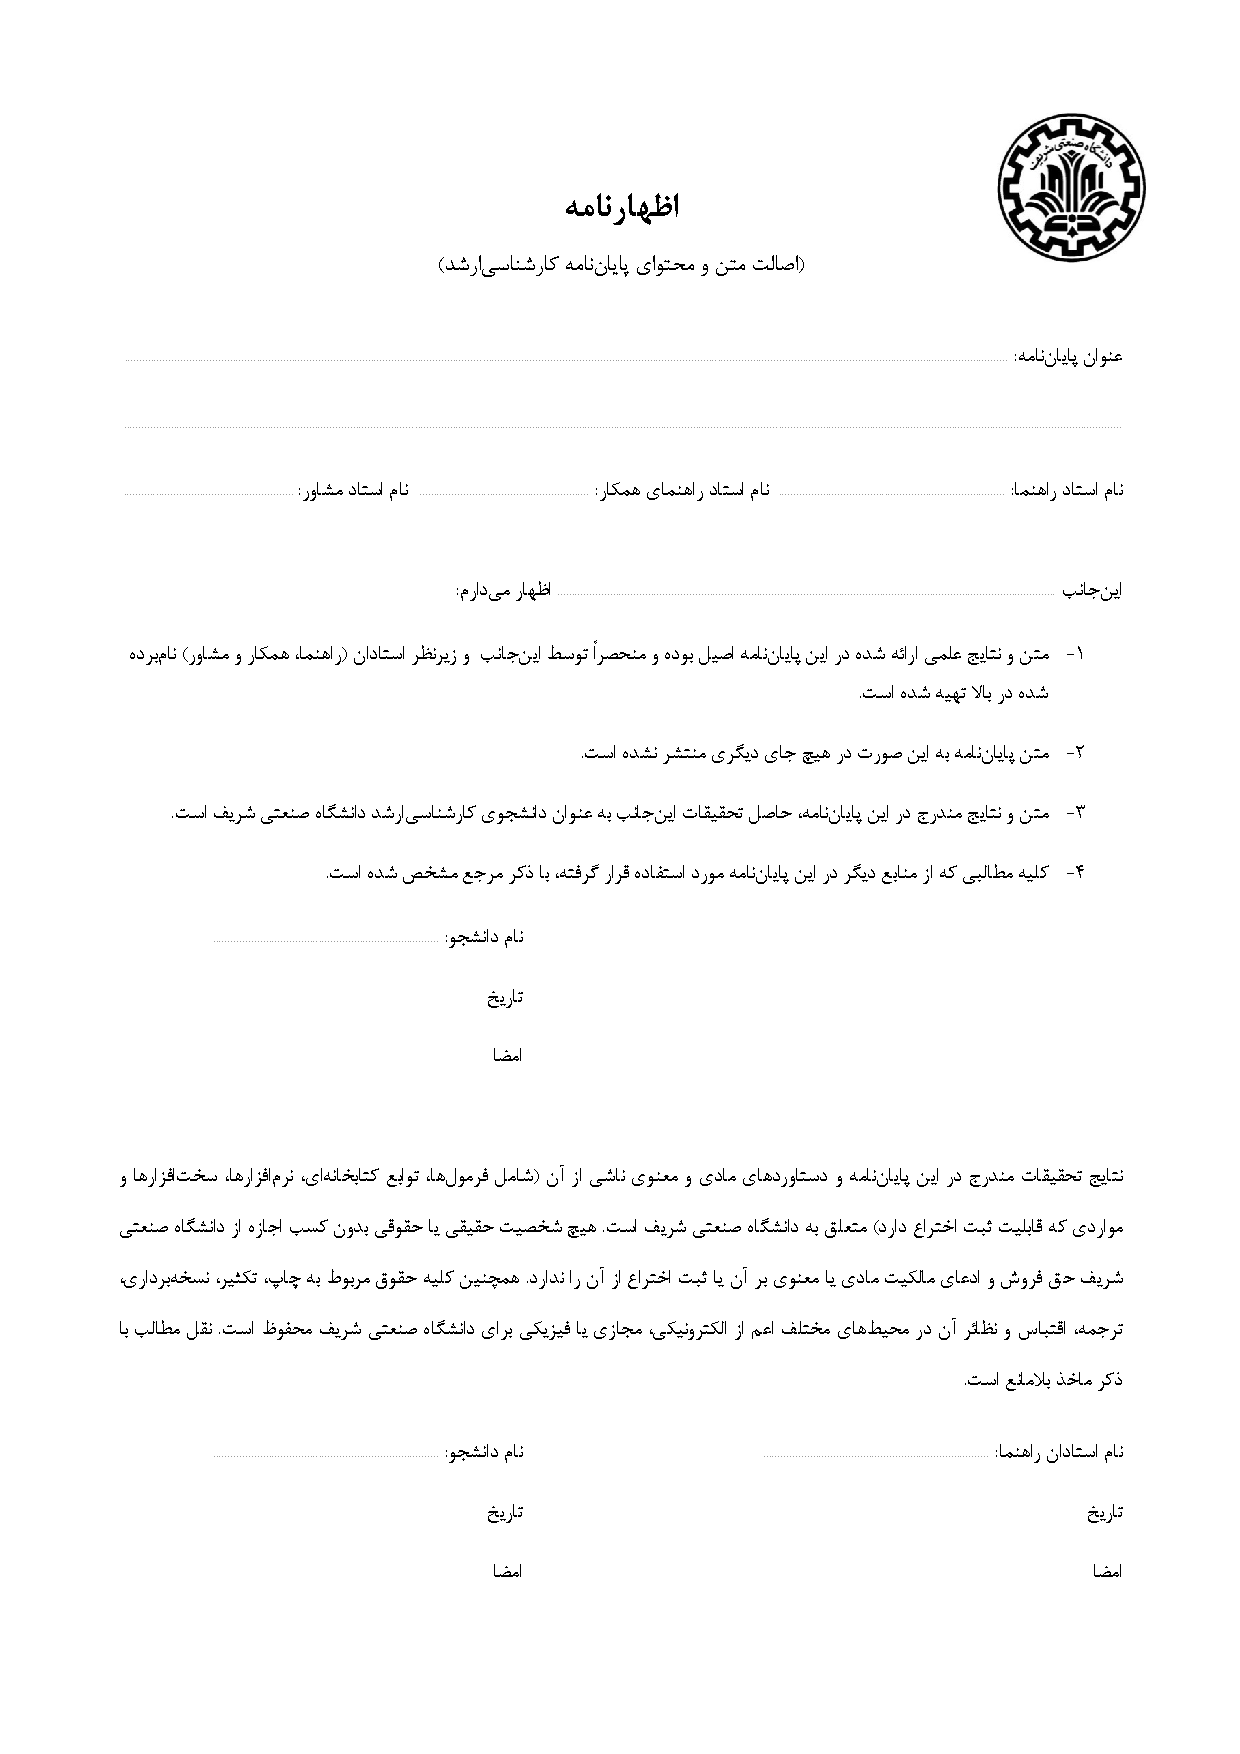
\includepdf[pages={1}]{Declaration.pdf}
	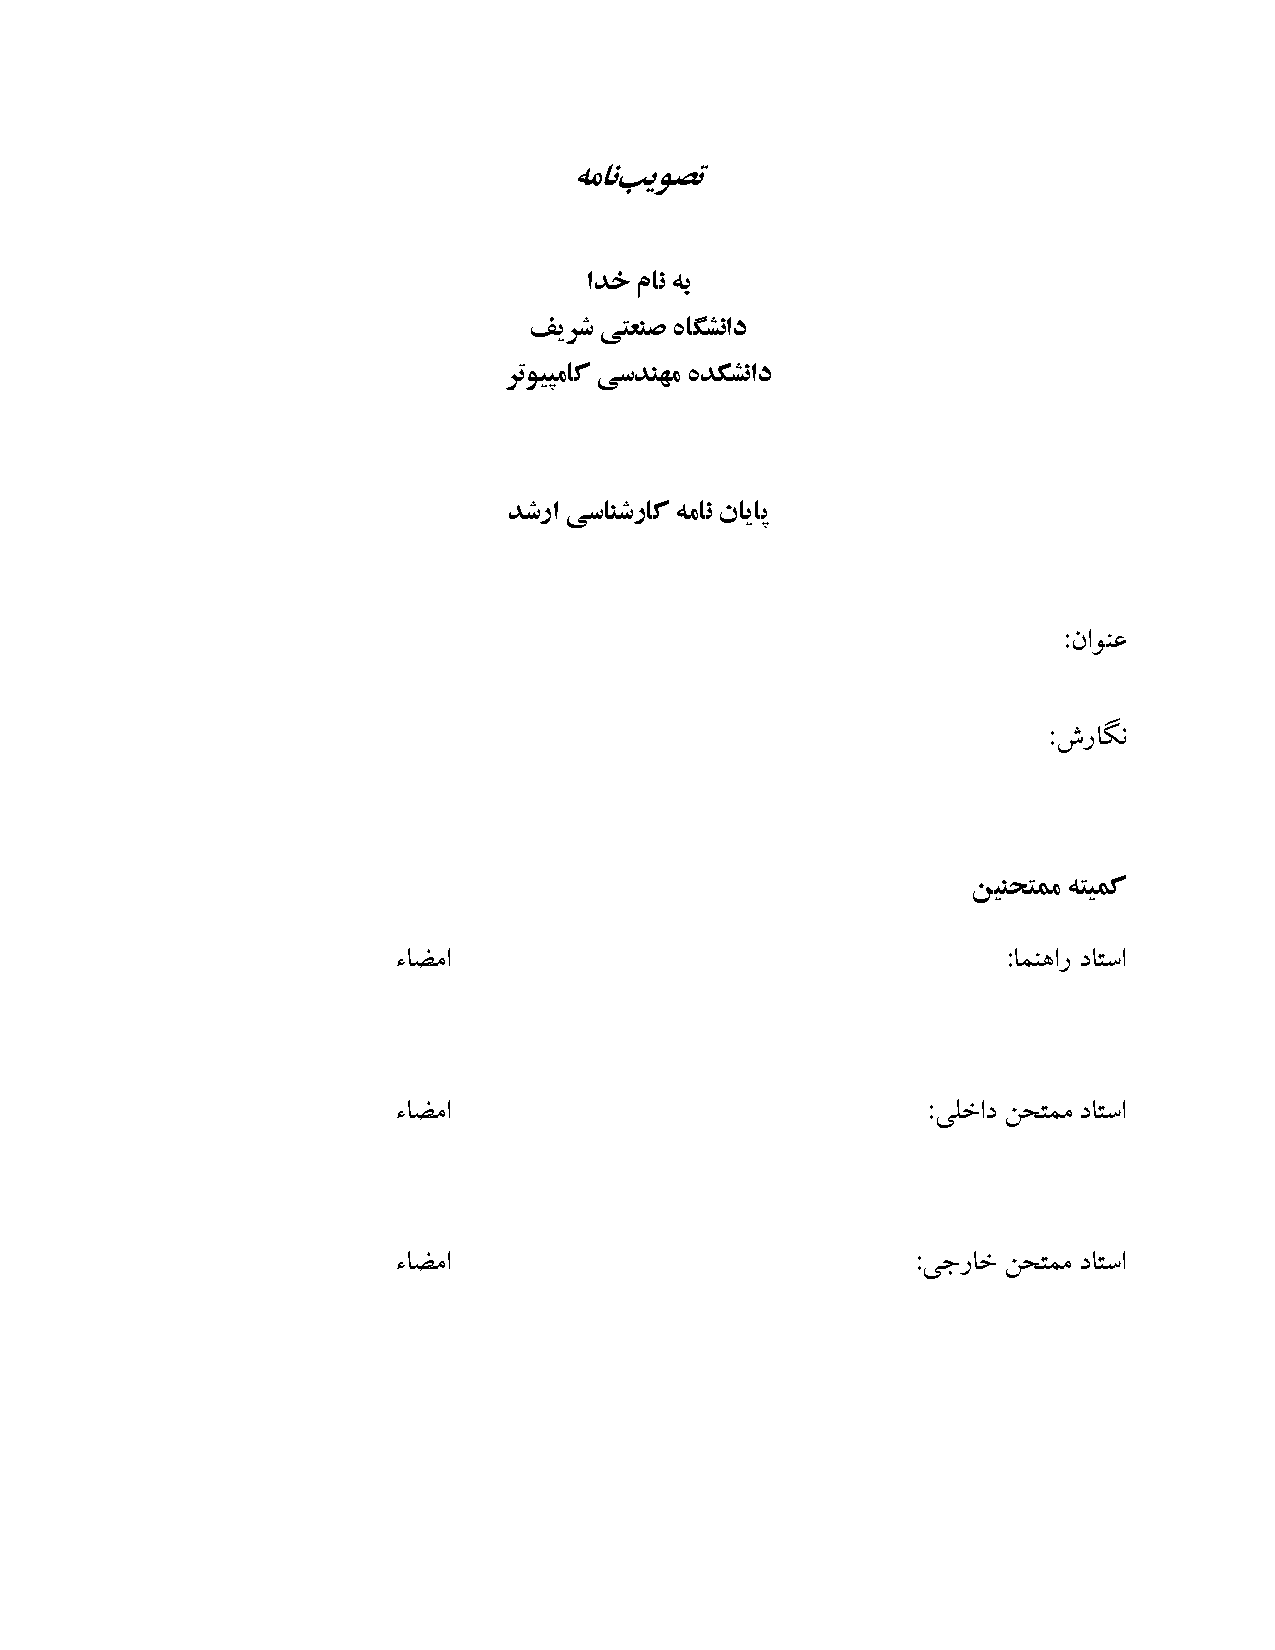
\includepdf[pages={1}]{ApprovalSheet.pdf}

	
	
% -------------------------------------------------------
%  Acknowledgments
% -------------------------------------------------------


اول از همه از استاد بزرگوارم دکتر کسائی به خاطر راهنمایی‌ها و کمک‌هایشان، چه در زمینه این تحقیق و چه خارج از آن، کمال تشکر و قدردانی را دارم. \\

همچنین از دوستان خوبم در آزمایشگاه پردازش تصویر به خاطر راهنمایی‌ها و لحظات خوشی که در طول یک سال اخیر برای بنده به‌وجودآورده‌اند تشکر بسیار دارم. \\

در نهایت از خانواده‌ی مهربانم سپاسگزارم که همانند سایر مراحل زندگی‌ام همواره حامی و پشتیبان من بوده‌اند، به خصوص خواهر عزیزم که در دوران تحصیلم همیشه راهنما، مشوق و همراه من بوده‌است.


\pagebreak

	
% -------------------------------------------------------
%  Abstract
% -------------------------------------------------------

\vspace*{-60pt}
\enlargethispage{90pt}

\شروع{وسط‌چین}
\مهم{چکیده}

\پایان{وسط‌چین}
\vspace{-1cm}

\بدون‌تورفتگی


ردیابی و ‌‌بازشناسایی موثر افراد برای تجزیه و تحلیل ویدیوهای ورزش تیمی امری ضروری است. این کار اما به دلیل حرکت غیرخطی بازیکنان در مقایسه با عابر پیاده، شباهت ظاهری بازیکنان یک تیم، فاصله دوربین از افراد حاضر در زمین و انسدادهای مکرر، کاملا چالش برانگیز است. بنابراین، توانایی استخراج بازنمایی‌های معنادار برای نمایش افراد در توسعه یک سیستم ردیابی و بازشناسایی موثر بسیار مهم است. در ورزش های تیمی اما، اطلاعات دیگری وجود دارد که می تواند در بازشناسایی افراد استفاده شود، مانند وابستگی‌تیم، اطلاعات نقش هر فرد و شماره پیراهن. با ظهور شبکه های عصبی پیچشی ژرف و پیشرفت آن‌ها در وظایف ورزشی، در حال حاضر شبکه‌های خوبی با دقت بالا برای وظایف گفته شده وجود دارد. با این حال، روش‌های موجود معمولاً از دو مشکل رنج می‌برند: اول، آموزش شبکه‌های مجزا برای هر یک از آن وظایف با هزینه‌های محاسباتی بالایی همراه است، و دوم، انسدادهای سنگین و ظاهر مشابه در ویدیوهای ورزشی، که دقت راه‌حل‌های موجود برای این کارها را محدود می‌کند. در این پژوهش، یک روش بازنمایی فرد پاره-محور چند منظوره به نام $PRTreID$ پیشنهاد شده است که سه وظیفه دسته‌بندی نقش، وابستگی‌تیم و بازشناسایی را به طور همزمان انجام می‌دهد. برخلاف کارهای موجود، یک شبکه واحد با نظارت چند وظیفه‌ای برای حل هر سه کار به طور مشترک آموزش داده می شود که از نظر محاسباتی موثر است. روش پیشنهادی پاره-محور است و از اطلاعات مبتنی بر قسمت‌های مختلف بدن برای هر فرد بهره می‌برد که می‌تواند به طور قابل توجهی در فرنامه‌های انسداد مفید باشد. همانطور که توسط نتایج کمی و کیفی نشان داده شده‌است، یادگیری چند وظیفه‌ای منجر به بازنمایی های غنی تر و تمایز دهنده تر می‌شود. علاوه بر این، مدل $PRTreID$ پیشنهادی با یک روش ردیابی مبتنی بر بازشناسایی یکپارچه شده و یک الگوریتم پس‌پردازش پاره-محور برای مدیریت ردیابی بلند‌مدت پیشنهاد شده است. با مدل چندمنظوره بازشناسایی پیشنهادی، روش ردیابی به دست آمده، $PRT-Track$، قادر است به طور موثر افراد را حتی در فرنامه‌های چالش برانگیز ردیابی کند، و از همه روش های ردیابی اخیر در مجموعه‌داده چالش برانگیز $SoccerNet-Tracking$ بهتر عمل‌کند. روش پیشنهادی معیارهای $HOTA$ و $AssA$ را نسبت به بهترین روش موجود، به ترتیب، به مقدار $1.57$ و $2.53$ درصد بهبود می‌دهد.



\پرش‌بلند
\بدون‌تورفتگی \مهم{کلیدواژه‌ها}: 
بینایی کامپیوتر، یادگیری ژرف، ویدیوهای ورزش تیمی، بازشناسایی، ردیابی چندشیء، بازشناسایی پاره-محور، وابستگی‌تیم، یادگیری چندوظیفه‌ای، یادگیری بازنمایی 
\صفحه‌جدید

	
	
	% -------------------- Table of Contents --------------------
	
	\pagestyle{fancy}
	
	\dominitoc
	\tableofcontents \newpage
	\listoffigures \newpage
	\listoftables \newpage
	%\let\clearpage
	%\let\clearpage


	
	\pagenumbering{arabic}
	
	% -------------------- Chapters --------------------
	
	\فصل{مقدمه}



‫\قسمت{مقدمه}





‫\قسمت{ تعريف و اهمیت مسئله و کاربرد‌های آن}




\قسمت{چالش‌ها}




‫\قسمت{هدف پژوهش}


‫\قسمت{دستاورد‌های پژوهش}

مشارکت‌های\پاورقی{contributions} این پژوهش به صورت زیر خلاصه می‌شود:

‫‫‫\شروع{فقرات}


\فقره ارائه یک روش ردیابی افراد با استفاده از ویژگی‌های مبتنی به بخش و یک روش پس‌پردازش پاره-محور برای حل مسئله ردیابی بلند مدت.



\پایان{فقرات}

‫

‫
‫\قسمت{ساختار پایان‌نامه}


\newpage
	\فصل{ادبیات پژوهش}



\قسمت{مقدمه}


\قسمت{ردیابی چندشیء}



\begin{figure}[htbp]
	\centering
	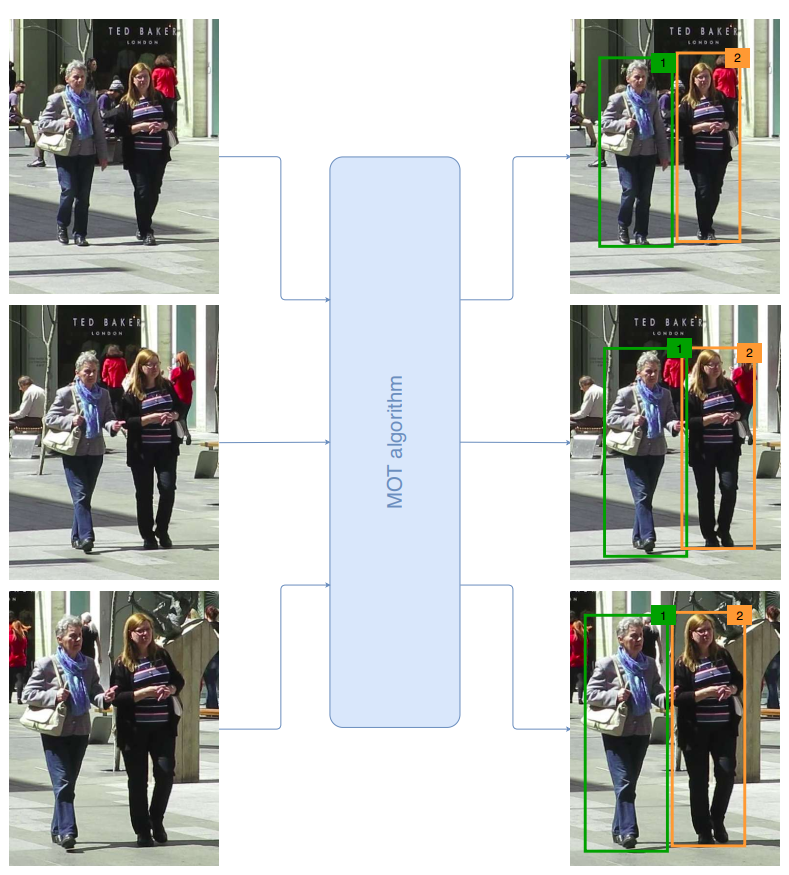
\includegraphics[scale=0.6]{figures/1_MOT_Diagram.png}
	\captionsetup{justification=centering}
	\caption[نمای کلی یک الگوریتم ردیابی]{نمای کلی یک الگوریتم ردیابی. ورودی شامل یک ویدیو بوده که از تعدادی قاب تشکیل شده‌ا	ست.  در خروجی در هر قاب برای هر شیء (فرد) یک جعبه‌مرزی  و یک شماره به عنوان شناسه آن در طول ویدیو بدست می‌آید\cite{ciaparrone2020deep}.}
	\label{1_MOT_Diagram}
\end{figure}




\قسمت{جمع‌بندی}

\newpage
	\فصل{روش‌پیشنهادی}


‫\قسمت{مقدمه و شرح روش به‌ صورت‌ كلی}





‫\قسمت{بازنمایی چند‌منظوره فرد پاره-محور}






‫‫\قسمت{جمع‌بندی}



	
\فصل{ارزیابی}

\label{section:experiment}
\قسمت{مقدمه}


\قسمت{مجموعه‌داده}




\قسمت{‌معیارهای ارزیابی}


\قسمت{‌جزئیات پیاده‌سازی}


\قسمت{‌نتایج تجربی}



\subsection{مقایسه با کار‌های پیشین}



\subsection{مطالعات فرسایشی}




‫‫\قسمت{جمع‌بندی}


\begin{table*}[!htbp]
	\caption[نتایج ردیابی]{نتایج ردیابی. مقایسه عملکرد روش پیشنهادی $PRT-Track$ و روش‌های ردیابی اخیر بر روی مجموعه تست مجموعه‌داده ردیابی $Soccernet-Tracking$. (نماد $\dagger$ به معنای این است که نتایج گزارش شده از \cite{cioppa2022soccernet} است.)}
	\begin{center}
		\begin{tabular}{ |c|c|c|c|c|c|c| } 
			\hline
			\multicolumn{7}{|c|}{truth ground using detections Oracle} \\
			\hline
			Method  & HOTA $\uparrow$ & DetA $\uparrow$ &  AssA $\uparrow$ & MOTA $\uparrow$ &  1IDF $\uparrow$ &  IDs $\downarrow$ \\
			\hline
			DeepSORT$^{\dagger}$ &   $69.52$ & $82.62$ & $58.66$ & $94.84$ & - & - \\ 
			
			ByteTrack$^{\dagger}$  & $71.5$ & $84.34$ & $60.71$ & $94.57$ & -  & - \\ 
			
			OC-SORT  &$ 80.94$ & $97.81$ & $66.98$ & $96.76$ & $74.79$ & $6079$  \\ 
			
			StrongSORT  &  $83.75$ & $95.08$ & $73.78$ & $94.67$ & $79.13$ & $2815$ \\ 
			
			StrongSORT++  &  $84.08$ & $95.07$ & $74.36$ & $94.62$ & $79.76$ & \textbf{$2619$} \\ 
			
			CBIoU  &  $89.20$ & $99.40$ & $80.00$ & $99.40$ & $86.10$ & -\\ 
			
			\textbf{PRT-Track} &  \textbf{$90.77$} & \textbf{$99.83$} & \textbf{$82.53$} & \textbf{$98.66$} & \textbf{$88.47$} & $3355$\\ 
			
			\hline
			\hline
			\multicolumn{7}{|c|}{detections 8YOLOv } \\
			\hline
			Method  & HOTA $\uparrow$ & DetA $\uparrow$ &  AssA $\uparrow$ & MOTA $\uparrow$ &  1IDF $\uparrow$ &  IDs $\downarrow$ \\
			\hline
			DeepSORT$^{\dagger}$  & $36.63$ & $40.02$ & $33.76$ & $33.91$ & -  & -\\ 
			
			FairMOT$^{\dagger}$  & $43.91$ & $46.31$ & $41.77$ & $50.69$ & - & -\\ 
			
			ByteTrack$^{\dagger}$  &  $47.22$ & $44.49$ & $50.25$ & $31.74$ & -  & -\\ 
			
			OC-SORT  &  $54.60$ & \textbf{$63.47$} & $47.07$ & \textbf{$76.18$} & $62.52$  & 3593\\ 
			
			StrongSORT  &  $54.86$ & $62.19$ & $48.79$ & $74.52$ & $65.1$ & $2178$\\ 
			
			StrongSORT++ & $56.21$ & $62.89$ & $50.27$ & $75.02$ & $66.53$ & $2106$\\ 
			
			\textbf{PRT-Track} &  \textbf{$59.77$} & $61.09$ & \textbf{$58.55$} & $73.07$ & \textbf{$74.44$} & \textbf{$1428$} \\ 
			\hline
			
		\end{tabular}
		\label{4_tracking_results}
	\end{center}
\end{table*}


\pagebreak
	
\فصل{جمع‌بندی و كارهای آتی}
در این بخش ابتدا یک جمع‌بندی از کار‌های انجام‌شده در این پژوهش ارائه‌می‌شود. در ادامه به کار‌هایی که می‌تواند در آینده در ادامه پژوهش فعلی انجام‌شود بررسی می‌شود.
‫
‫
\قسمت{جمع‌بندی و نتیجه‌گیری}

‫
‫
\قسمت{کارهای آتی}





\pagebreak
	
	% -------------------- Appendices --------------------
	
	\begin{appendix}
		\vspace{-1cm}
\فصل{مطالب و نتايج تکمیلی }
\vspace{-1cm}



\pagebreak
	\end{appendix}
	
	% -------------------- Bibliography --------------------
	
	
	
% -------------------------------------------------------
%  Bibliography
% -------------------------------------------------------


\begin{latin}
\baselineskip=.8\baselineskip
\bibliographystyle{./styles/packages/unsrtabbrv}

% Uncomment next line to include uncited references
% \nocite{*}

\bibliography{bibs/full,bibs/refs}
 
\end{latin}
\newpage

	
	
	% -------------------- English Pages --------------------
	
	
	\newgeometry{left=3cm,right=2.5cm}
	
	
\rhead{واژه‌نامه}

\chapter*{واژه‌نامه}
\begin{multicols}{2}
\small

\dicalphabet{الف}
\dic{occlusion}{انسداد}
\dic{detection}{آشکارسازی}
\dic{confidence}{اطمینان}
\dic{concatenate}{الحاق}
\dic{promising}{امیدوار‌کننده}
\dic{triplet loss}{اتلاف سه‌گانه}
\dic{inference}{استنتاج}
\dic{threshold}{آستانه}
\dic{ent-to-end}{انتها‌به‌انتها}


\dicalphabet{ب}
\dic{recognition}{بازشناسی}
\dic{offline}{برون‌خط}
\dic{retrieval}{بازیابی}
\dic{label}{برچسب}
\dic{embedding}{بازنمایی}
\dic{augmentation}{برافزایی}




\end{multicols}

\newpage

	
% -------------------------------------------------------
%  English Abstract
% -------------------------------------------------------


\pagestyle{empty}

\begin{latin}

\begin{center}
\textbf{Abstract}
\end{center}
\baselineskip=.8\baselineskip

english abstract.


\bigskip\noindent\textbf{Keywords}:
Computer Vision, Deep Learning
\end{latin}

\newpage

	
\pagestyle{empty}

\begin{center}

\begin{latin}

\includegraphics[scale=0.2]{front/template/images/logo.png}

\EnglishThesisUniversity \\
\EnglishThesisDepartment

\begin{large}
\vspace{0.7cm}
\EnglishThesisType


\vspace{1.5cm}

{\Large\textbf\EnglishThesisTitle}

\vspace{1.5cm}

{\normalsize By:}\\
\textbf{\EnglishThesisAuthor}

\vspace{1cm}

{\normalsize Supervisor:}\\ 
\textbf{\EnglishThesisSupervisor}

\end{large}

\vspace{1.5cm}
\EnglishThesisDate

\end{latin}

\end{center}

	
	% -------------------- The End! --------------------
	
\end{document}
